\section{Teoremi generali}
Questa sezione vuole raccogliere alcuni teoremi importanti che però non appartengono a nessuna sezione precedente in particolare in quanto richiedono l'uso di molti argomenti presi da sezioni differenti. Ho quindi congegnato che era meglio dedicare loro una sezione a parte, sperando che il mio intento di organizzazione possa essere apprezzato da quelli che leggeranno.

\subsection{Teorema degli zeri}
Il teorema degli zeri è estremamente importante in analisi. In pratica afferma che se una funzione è continua e ha un punto in cui è positiva (quindi è sopra l'asse delle ascisse) e un punto in cui è negativa (quindi è sotto l'asse delle ascisse), per forza tra quei due punti ce ne sarà un terzo in cui la funzione tocca l'asse delle ascisse. È abbastanza facile verificare che è vero in quanto se si vuol tracciare una linea continua che in punto è sopra l'asse delle ascisse e in un altro è sotto, per forza si è costretti ad intersecare tale asse.
\begin{figure}[h]
    \centering
    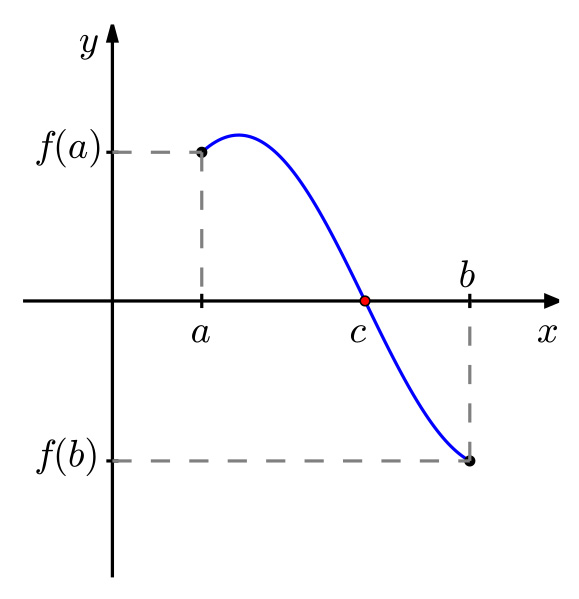
\includegraphics[width=180px]{../img/TeoremaZeri.jpg}
    \caption{Rappresentazione grafica del teorema degli zeri}
\end{figure}
Per dimostrare questo teorema abbiamo però bisogno di due lemmi preliminari:

\mlem{
Data una successione $(a_n)_n \subseteq \mathbb{R}$ , se 
\begin{equation*}
    \forall n, a_n < 0 \implies \lim _{x \to +\infty} a_n = l \in R \; \land \; l \leq 0
\end{equation*}
Si noti che questo lemma vale anche per il caso in cui $\forall n, a_n > 0$, che implica $l \geq 0$. Dimostriamo ora il lemma\footnote{La seguente dimostrazione è stata fatta dal prof in maniera imbarazzante, quindi la esplicito secondo la logica classica per renderla più formale}. Dobbiamo provare che:
\begin{equation*}
    \forall n, a_n < 0 \implies \lim _{x \to +\infty} a_n = l \leq 0
\end{equation*}
Fisso $n$ numero t.c $\forall n, a_n < 0$ (H) per dimostrare:
\begin{equation*}
    \lim _{x \to +\infty} a_n = l \leq 0
\end{equation*}
Per assurdo assumiamo\footnote{Abbiamo usato il potere sconfinato della RAA (Coen approves)} $l > 0$ (H2) e riduciamoci a dimostrare il falso. Grazie alla definizione di limite possiamo riscrivere il limite nel seguente modo:
\begin{equation*}
    \forall \epsilon > 0, \exists \overline{n} \in \mathbb{N} : \forall n \geq \overline{n} \implies |q_n - l| < \epsilon
\end{equation*}
Se espandiamo $|q_n - l| < \epsilon$ ci troviamo con:
\begin{equation*}
    l - \epsilon < a_n < l + \epsilon
\end{equation*}
Ed essendo che questa condizione delle valere $\forall \epsilon > 0$, scegliamo $\epsilon = \dfrac{l}{2}$. Quindi deve valere che:
\begin{equation*}
    a_n > l - \epsilon = l - \dfrac{l}{2} = \dfrac{l}{2}
\end{equation*}
Per (H2) $\dfrac{l}{2} > 0$ ma per (H) $\forall n, a_n < 0$. ASSURDO in quanto $a_n$ non può contemporaneamente essere maggiore di $0$ e minore di $0$.\\

\hfill Qed.
}

\mlem{
Data una funzione $f: A \to \mathbb{R}$, un punto $x_0 \in A \cap \mathcal{D}(A)$ e inoltre $f$ deve essere continua in $x_0$:
\begin{equation*}
    \forall (a_n)_n \subseteq A : a_n \to x_0 \implies f(a_n) \xrightarrow[n \to + \infty]{} f(x_0)
\end{equation*}
}

\thm {
\begin{equation*}
f:[a,b] \to \mathbb{R}\;\; \text{continua, }\; f(a) \cdot f(b) < 0 \implies \exists c \in ]a,b[ : f(c) = 0
\end{equation*}
}
Un paio di osservazioni utili sul teorema:
\begin{itemize}
    \item La continuità di $f$ è fondamentale in quanto se non lo fosse il teorema non potrebbe valere. Si consideri infatti il caso di una funzione definita a tratti nel seguente modo:
    \begin{equation*}
        f(x) =
        \begin{cases*}
            -1 \qquad (0 \leq x \leq 2)\\
            1   \qquad \;\;\;(2 < x \leq 4)
        \end{cases*}
    \end{equation*}
    Quest'ultima rispetta tutte le specifiche del teorema ($f(0) \cdot f(4) < 0$) tranne la continuità (non è infatti continua in $x = 2$). Se si osserva il grafico (Figura: \ref{fig_teoraZeri}) si nota subito che questa funzione non ammette nessun punto in cui si annulla come vorrebbe il teorema degli zeri.

    \begin{figure}[h]
        \centering
	\begin{tikzpicture}
	\begin{axis}[xmax = 4, xmin = -1.5, ymax = 2, ymin = -2,
			axis lines=middle, xlabel=$x$, ylabel=$y$,
			     xtick={-1, 0, 1, 2, 3, 4, 5, 6},
			     ytick={-1, 1},
			     xlabel style={anchor=north east},
			     xticklabel style={anchor=north},
			     yticklabel style={anchor=east},
			    ]
		\addplot[domain=0:2, samples=200]{-1};
		\addplot[domain=2:4, samples=200]{1};
		\addplot [only marks, mark options={scale=1.5}] table {
		2 1
		2 -1
		};
		\addplot [only marks, white] table {
		2 1
		};
	\end{axis}
	\end{tikzpicture}


	\caption{Funzione definita a tratti per far vedere che la continuità nel teorema degli zeri è una condizione necessaria}
        \label{fig_teoraZeri}
    \end{figure}

    \item La seconda osservazione riguarda la quantità di punti in cui si può annullare la funzione. Come si legge dal teorema, il punto $c$ è garantito che esista ($\exists$) ma nessuno garantisce che è unico. Ci possono essere infatti un numero arbitrario di punti in cui la funzione si annulla, basti pensare al grafico delle funzioni goniometriche $\sin(x)$ e $\cos(x)$.
\end{itemize}


\pf{
  Questa dimostrazione a differenza delle altre è di tipo \textit{costruttivo}, cioè oltre a dimostrare il teorema fornisce un algoritmo di calcolo per trovare il punto $c$.\\

  Assumiamo $f(a) < 0$ e $f(b) > 0$. 
  L'idea dietro questa dimostrazione è appunto trovare un algoritmo di calcolo che permetta di determinare il punto $c$. Avendo un punto $a$ in cui la funzione è \textbf{negativa} e un punto $b$ in cui la funzione è \textbf{positiva} ci deve essere un punto che giace tra $a$ e $b$ in cui la funzione si annulla. Per trovarlo andiamo a "tentativi" dividendo l'intervallo a metà con la formula:
  \begin{equation*}
    \dfrac{a+b}{2}
  \end{equation*}
  Da qui possiamo avere 3 casi:
  \begin{enumerate}
    \item $f\left(\dfrac{a + b}{2}\right) = 0$. In questo caso abbiamo trovato il punto $c$ proprio perché la funzione si annulla. Quindi abbiamo finito!
      \begin{equation*}
        c = \dfrac{a+b}{2}
      \end{equation*}

      \item $f\left(\dfrac{a + b}{2}\right) < 0$. In questo caso non abbiamo trovato il punto $c$, ma bensì la funzione ci ha restituito un punto negativo. Essendo il punto $f(b)$ ancora maggiore di $0$ per ipotesi, possiamo applicare nuovamente questa procedura (cioè di suddividere l'intervallo a metà), però cambiando il punto $a$, in quanto adesso diventa:
      \begin{equation*}
        a_2 := \dfrac{a+b}{2}
      \end{equation*}

    \item $f\left(\dfrac{a + b}{2}\right) > 0$. L'idea di questo punto è identica a quella del punto 2, semplicemente invece che assegnare un valore diverso ad $a$, lo assegniamo a $b$ perché questa volta il valore della funzione è positivo invece che negativo.
      \begin{equation*}
        b_2 := \dfrac{a+b}{2}
      \end{equation*}
  \end{enumerate}
  Con i punti 2 e 3, riassegnando il valore ad $a$ o $b$, restringiamo l'intervallo su cui vogliamo applicare questo algoritmo per trovare il punto $c$. Ed essendo che ad ogni iterazione ci avviciniamo sempre di più, a forza di stringere l'intervallo prima o poi arriveremo a $c$.\\
  \textbf{Nota:} Ad ogni iterazione, se la funzione non si annulla, dobbiamo sostituire il valore del punto al corrispettivo punto $a$ o $b$ in modo che la funzione mantenga lo stesso segno. Questo perché se invertissimo i punti ci troveremmo in un caso in qui $f(a) > 0$ e $f(b) > 0$, cosa che ovviamente annullerebbe il teorema. Quindi nel caso del punto 2 in cui sostituiamo il nuovo punto ad $a$, lo facciamo soltanto perché per ipotesi $f(a) < 0$ e la funzione nel nuovo punto è negativa. Se per ipotesi avessimo scelto $f(a) > 0$ avremmo dovuto sostituire il nuovo punto in $b$, e viceversa.\\

  Essendo che dobbiamo ripete l'algoritmo, il caso \textit{n}-ario diventa:
  \begin{enumerate}
    \item 
      \begin{equation*}
        f\left(\dfrac{a_n + b_n}{2}\right) = 0 \;\; \qquad \qquad \qquad \text{Fine:} \;\; \qquad \qquad \qquad c = \dfrac{a_n + b_n}{2}
      \end{equation*}

    \item 
      \begin{equation*}
        f\left(\dfrac{a_n + b_n}{2}\right) < 0 \qquad \text{Iteriamo nuovamente:} \qquad a_{n + 1}:= \dfrac{a_n + b_n}{2}
      \end{equation*}
      
    \item 
      \begin{equation*}
        f\left(\dfrac{a_n + b_n}{2}\right) > 0 \qquad \text{Iteriamo nuovamente:} \qquad b_{n + 1}:= \dfrac{a_n + b_n}{2}
      \end{equation*}

  \end{enumerate}

  Se l'algoritmo termina al passo $p \in \mathbb{N}$ significa che:
  \begin{equation*}
    f\left(\dfrac{a_p + b_p}{2}\right) = 0 \qquad \text{e quindi:} \qquad c = \dfrac{a_n + b_n}{2}
  \end{equation*}
  Altrimenti la procedura non termina: in questo caso avremo costruito due successioni $(a_n)_n$ e $(b_n)_n$ contenute in $[a, b]$. Scriviamo di seguito le proprietà di queste 2 successioni:
  \begin{enumerate}[label=\roman*.]
    \item $a_n \leq a_{n+1} \forall n \in \mathbb{N}$ \quad e \quad $b_n \leq b_{n+1} \forall n \in \mathbb{N}$

    \item $a_n \leq b_n \forall n \in \mathbb{N}$ 
      
    \item $f(a_n) < 0, \;\; f(b_n) > 0 \quad \forall n \in \mathbb{N}$
    
    \item 
      \begin{equation*}
        b_n - a_n = \dfrac{b_{n-1} - a_{n-1}}{2} \qquad \forall n
      \end{equation*}
      Se si espandono i vari passaggi si vede che in realtà ad ogni iterazione si divide l'intervallo iniziale $[a, b]$ in 2:
      \begin{equation*}
        b_n - a_n = \dfrac{b_{n-1} - a_{n-1}}{2} = \dfrac{b_{n-2} - a_{n-2}}{2^2} = \dfrac{b_{n-2} - a_{n-2}}{2^3}  = \cdots = \dfrac{b_1 - a_1}{2^{n-1}}
      \end{equation*}
  \end{enumerate}

  A questo punto vogliamo dimostrare che:
  \begin{equation*}
    \begin{cases*}
      \lim \limits_{n \to +\infty} a_n = \lim \limits_{n \to +\infty} b_n = c\\
      \\
      f(c) = 0
    \end{cases*}
  \end{equation*}
    Dal punto (i) e (ii) ricaviamo che sia $(a_n)_n$ sia $(b_n)_n$ sono \textbf{limitate}.
    \begin{equation*}
      (a_n)_n \subseteq [a, b] \implies a_n \nearrow \; \forall n \implies \exists \lim_{n \to +\infty} a_n = \alpha \in \mathbb{R}
    \end{equation*}
    \begin{equation*}
      (b_n)_n \subseteq [a, b] \implies b_n \nearrow \; \forall n \implies \exists \lim_{n \to +\infty} b_n = \beta \in \mathbb{R}
    \end{equation*}
    Dal punto (iv) e da quanto abbiamo ricavato possiamo fare il limite che tende a $+\infty$ di $b_n - a_n$:
    \begin{align*}
      \lim_{n \to +\infty} b_n - a_n &= \lim_{n \to +\infty} \dfrac{b_1 - a_1}{2^{n-1}}\\
      \beta - \alpha &= 0
    \end{align*}
    Quindi $\beta = \alpha$ e le due successioni hanno lo stesso limite! Abbiamo quindi provato che:
    \begin{equation*}
      \lim \limits_{n \to +\infty} a_n = \lim \limits_{n \to +\infty} b_n := c
    \end{equation*}
    Ci resta da dimostrare che $f(c) = 0$. Da quanto appena dimostrato e dal primo lemma di questa prova:
    \begin{equation*}
      \lim \limits_{n \to +\infty} f(a_n) = f(c)
    \end{equation*}
    Poiché $a_n \to c$. Inoltre dal punto (iii) sappiamo che $f(a_n) < 0 \; \forall n \in \mathbb{N}$. Usando il secondo lemma preliminare alla prova:
    \begin{equation*}
      f(c) \leq 0
    \end{equation*}
    Se facciamo lo stesso per $f(b_n)$:
    \begin{equation*}
      \lim \limits_{n \to +\infty} f(b_n) = f(c) \geq 0
    \end{equation*}
    Avendo contemporaneamente $f(c) \leq 0$ e $f(c) \geq 0$:
    \begin{equation*}
      f(c) = 0
    \end{equation*}
    \hfill Qed.
}

\subsection{Radici di un polinomio di grado dispari}

\thm{
Ogni polinomio di grado dispari ha almeno un radice reale.
}
È facile ricordarsi questo teorema perché tutti i polinomi di grado dispari hanno il termine di grado maggiore (che in quanto dispari) è soggetto al segno dell'argomento del polinomio. Cioè $x^3$ avrà lo stesso segno di $x$, mentre questo non vale per i polinomi di grado pari in quanto $x^8$ avrà sempre segno positivo. Se quindi si fanno i limiti per $+\infty$ e $-\infty$ di un polinomio di grado dispari, da una parte andrà sempre a $+\infty$ e dall'altra andrà sempre a $-\infty$ (seguendo appunto il segno della $x$). Ed essendo inoltre i polinomi funzioni continue, sono costretti ad assumere tutti i valori dell'asse delle ordinate almeno una volta\footnote{Per chiarire: non assumono tutti i valori dell'asse delle ordinate perché sono funzioni continue e basta, assumono tutti i valori perché sono funzioni continue su $\mathbb{R}$ e da una parte vanno a $+\infty$ e dall'altra a $-\infty$}. Inoltre, visto che da una parte hanno valori positivi, dall'altra negativi e sono continui, esiste per forza un punto in cui si annullano (dal teorema degli zeri) e sarà proprio lì la loro radice.\\

\textbf{Corollario:}
Tutti i polinomi di grado dispari assumono \textbf{tutti i valori reali}. Questo implica che una funzione che è definita tramite un polinomio di grado dispari è una funzione \textbf{suriettiva}, in quanto ha come immagine $\mathbb{R}$.
\pf{
  Dimostrazione del corollario:\\

  Preso un qualsiasi polinomio di \textbf{grado dispari} $p(x)$, dobbiamo dimostrare che assume tutti i valori reali, cioè:
  \begin{equation*}
    \forall k \in \mathbb{R} \;\; p(x) = k \;\; \text{ha almeno una soluzione}
  \end{equation*}
  Ci basta considerare l'equazione $p(x) - k = 0$ (che resta un generico polinomio di grado dispari) e applicare il teorema appena enunciato.\\

  \hfill Qed.
}

\subsection{Teorema di Weierstrass} % Di questo teorema ho due formulazioni perché la seconda si basa sulla prima e sul teorema degli zeri. Non so se sono effettivamente importanti entrambe, però sono leggermente diverse tra loro (la seconda è più generale) e quindi ho deciso di scriverle entrambe.
\label{theorem_weierstrass}
\dfn {
$f:A \to \mathbb{R}$
\begin{enumerate}
    \item $x_0 \in A$ si dice punto di \textbf{massimo assoluto} di $f$ se:
    \begin{equation*}
        f(x) \leq f(x_0) \quad \forall x \in A
    \end{equation*}
    
    \item $x_0 \in A$ si dice punto di \textbf{minimo assoluto} di $f$ se:
    \begin{equation*}
        f(x_0) \leq f(x) \quad \forall x \in A
    \end{equation*}
\end{enumerate}
}

\subsubsection{Formulazione 1} 

\thm{
Una funzione continua, in un intervallo chiuso e limitato, ammette il massimo e il minimo assoluti della funzione.\\
$f: [a,b] \to \mathbb{R}$ continua, allora:
\begin{equation*}
    \exists x_0 \in [a,b]: f(x) \leq f(x_0) = \vcentcolon M \quad \forall x \in [a,b]
\end{equation*}
\begin{equation*}
    \exists x_1 \in [a,b]: f(x) \leq f(x_1) = \vcentcolon m \quad \forall x \in [a,b]
\end{equation*}
E quindi:
\begin{equation*}
  \mathrm{Im}f([a,b]) \subseteq [m, M]
\end{equation*}
Cioè, l'immagine di $f$ in $[a, b]$ è un sottoinsieme dell'intervallo $[m, M]$.
}
È molto importante che la funzione sia \textit{continua}, \textit{in un intervallo chiuso} e \textit{limitato} perché se manca anche solo una di queste cose \textbf{non esiste} il minimo, il massimo o entrambi (come si vede dai grafici nelle figure: \ref{fig_weierstrassIntervalloAperto},  \ref{fig_weierstrassIntervalloIllimitato} e \ref{fig_weierstrassNonContinuo})

\begin{figure}[h]
\centering
\begin{tikzpicture}
\begin{axis}[xmax = 1.5, xmin = -0.5, ymax = 10, ymin = -0.5,
             axis lines=middle, xlabel=$x$, ylabel=$y$,
             xtick={0.5, 1},
             ytick={2, 4, 6, 8},
             ylabel style={anchor=south east},
             xticklabel style={anchor=north},
             yticklabel style={anchor=east},
             width=0.6\linewidth,
            ]
\addplot[domain=0:1, samples=200]{1/x};
\addplot [only marks] table {
1 1
};
\end{axis}
\end{tikzpicture}
  \caption{Intervallo aperto $]0,1]$}
  \label{fig_weierstrassIntervalloAperto}
\end{figure}



\begin{figure}
\centering
\begin{subfigure}{0.49\textwidth}
\centering
\begin{tikzpicture}
\begin{axis}[xmax = 10, xmin = -0.5, ymax = 2, ymin = -0.5,
             axis lines=middle, xlabel=$x$, ylabel=$y$,
             xtick={2, 4, 6, 8},
             ytick={0.5, 1, 1.5},
             xlabel style={anchor=north east},
             xticklabel style={anchor=north},
             yticklabel style={anchor=east},
            ]
\addplot[domain=1:10, samples=200]{1/x};
\addplot [only marks] table {
1 1
};
\end{axis}
\end{tikzpicture}

  \caption{Intervallo illimitato $[1,+\infty[$}
  \label{fig_weierstrassIntervalloIllimitato}
\end{subfigure}
\begin{subfigure}{0.49\textwidth}
\centering
\begin{tikzpicture}
\begin{axis}[xmax = 8, xmin = -0.5, ymax = 2, ymin = -0.5,
             axis lines=middle, xlabel=$x$, ylabel=$y$,
             xtick={1, 2, 3, 4, 5, 6},
             ytick={0.5, 1, 1.5},
             xlabel style={anchor=north east},
             xticklabel style={anchor=north},
             yticklabel style={anchor=east},
            ]
\addplot[domain=1:2, samples=200]{-0.5 * x + 1.5};
\addplot[domain=2:4, samples=200]{0.4 * x + 0.2};
\addplot[domain=4:6, samples=200]{1};
\addplot [only marks, mark options={scale=1.5}] table {
1 1
2 0.5
2 1
4 1.8
4 1
6 1
};
\addplot [only marks, white] table {
2 0.5
4 1.8
};
\end{axis}
\end{tikzpicture}

  \caption{Funzione non continua} 
  \label{fig_weierstrassNonContinuo}
\end{subfigure}
\caption{Altri due esempi per il teorema di Weierstrass}
\end{figure}

\subsubsection{Formulazione 2} 
La seconda formulazione di questo teorema è più generale rispetto alla prima e utilizza il teorema degli zeri in combinazione con la prima formulazione di questo teorema.

\thm{
$f:[a,b]\to \mathbb{R}$ continua, allora:
\begin{equation*}
    \exists M = \max f([a,b])
\end{equation*}

\begin{equation*}
    \exists m = \min f([a,b])
\end{equation*}
e vale che l'immagine di $f$ nell'intervallo $[a,b]$ corrisponde esattamente a $[m, M]$:
\begin{equation*}
  f([a,b]) = [m, M]
\end{equation*}
}

\pf{
	\begin{center}
		\begin{tikzpicture}[scale=2]

		\begin{scope}
			\draw[->] (-0.5,0) -- (3,0) node[right] {$x$};
			\draw[->] (0,-0.5) -- (0,3) node[above] {$y$};
		\end{scope}

			\draw[-] (0,1) -- (1,1);
			\draw[-] (1,0) -- (1,1);
			\draw[-] (0,2) -- (2.5,2);
			\draw[-] (0,1.3) -- (2.5,1.3);
			\draw[-] (2.5,0) -- (2.5,2);

		\draw[very thin, fill] (1,0) circle (0.4pt) node[right, yshift=6pt] {$x_1$}; %Punto
		\draw[very thin, fill] (2.5,0) circle (0.4pt) node[right, yshift=6pt] {$x_2$}; %Punto
		\draw[very thin, fill] (0,1) circle (0.4pt) node[left, yshift=5pt] {$m$}; %Punto
		\draw[very thin, fill] (0,1.3) circle (0.4pt) node[left, yshift=5pt] {$y$}; %Punto
		\draw[very thin, fill] (0,2) circle (0.4pt) node[left, yshift=5pt] {$M$}; %Punto

	\end{tikzpicture}

	\end{center}


	%Chi mi assicura l'esistenza di questi due punti? Il teorema prima?

	\begin{equation*}
		\exists x_1 \in [a, b] : f(x_1) = \min f = m
	\end{equation*}
	\begin{equation*}
		\exists x_2 \in [a, b] : f(x_2) = \min f = M
	\end{equation*}
	Definiamo una funzione ausiliaria che $\forall y \in ]m, M[$:
	\begin{equation*}
		g:[x_1, x_2] \to \mathbb{R} \qquad g(x) = f(x) -y
	\end{equation*}

	Se quindi calcoliamo la funzione $g$ nei punti $x_1$ e $x_2$ diventa:
	\begin{align*}
		g(x_1) = f(x_1) -y &= m - y < 0 \\
		g(x_2) = f(x_2) -y &= M - y > 0 
	\end{align*}

	Applicando quindi il teorema degli zeri:
	\begin{equation*}
		\exists {x_0} \in ]x_1, x_2[ \subseteq [a, b] : g(x_0) \iff f(x_0) - y = 0 \iff f(x_0) = y \quad \forall y \in ]m, M[ %L'intervallo nel teorema è chiuso, mentre qui è aperto. Che vuol dire?
	\end{equation*}
	\hfill Qed.
}

